\documentclass[12pt,a4paper,twoside]{article}

\usepackage{fancyhdr}
\usepackage{lastpage}
\usepackage{a4wide} 
\usepackage{amsmath}
\usepackage{amssymb} 
\usepackage{graphicx}
\usepackage{color}
\usepackage{fancybox}
\usepackage{moreverb}
\usepackage[T1]{fontenc}
% \usepackage{hangcaption}
\usepackage{listings}
\usepackage[latin1]{inputenc}

%\fbox{}
%\shadowbox{}
%\doublebox{}
%\ovalbox{}
%\Ovalbox{}
%\shabox{}


% --- Logo Atos ---
%\makebox[\textwidth][l]{
%\raisebox{-15pt}[0pt][0pt]{
%\hspace{2.5cm}
%\includegraphics[scale=0.1]{Images/logo_atos.eps}
%}
%}
\title{Rapport de projet de fin d'�tudes}
\author{Nom et Pr�nom Etudiant}
\date{\today}

\pagestyle{headings}

\begin{document}
\lstset{ numbers=left, tabsize=3, frame=single, numberstyle=\ttfamily, basicstyle=\footnotesize} 
\thispagestyle{empty}

\begin{center}
\makebox[\textwidth][l]{
\raisebox{-8pt}[0pt][0pt]{
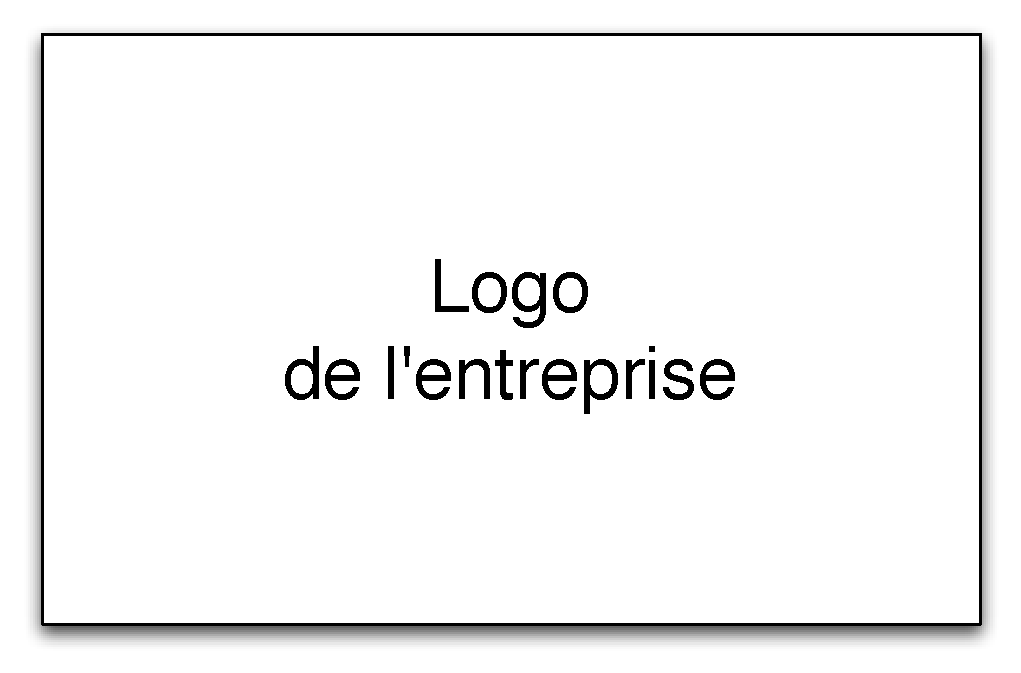
\includegraphics[scale=0.18]{Images/logo_entreprise}
}
}
\makebox[\textwidth][r]{
\raisebox{0pt}[0pt][0pt]{

\includegraphics[scale=0.2]{Images/logo_ensimag}
}
}
Grenoble INP  -- ENSIMAG\\
�cole Nationale Sup�rieure dInformatique et de Math�matiques Appliqu�es\\
\vspace{3cm}
{\LARGE Rapport de <type de stage> \\(Projet de Fin d'Etudes ou Stage Assistant-Ing�nieur)}\\
\vspace{1cm}
Effectu� chez Nom Entreprise\\
\vspace{2cm}
\shadowbox{
\begin{minipage}{1\textwidth}
\begin{center}
{\Huge Titre du Sujet de Stage}\\
\end{center}
\end{minipage}
}\\
\vspace{3cm}
Nom et Pr�nom Etudiant\\
<Ann�e de formation (1A, 2A ou 3A)> -- Option <intitul� de fili�re>\\
\vspace{3mm}
11 f�vrier 2008 -- 01 ao�t 2008\\
\vspace{3,5cm}
\begin{tabular}{p{10cm}p{10cm}}
{\bf Nom Entreprise}                                            &{\bf Responsable de stage}\\
{\footnotesize Adresse Entreprise}       & ~~~Nom Et Pr�nom Tuteur Entreprise\\
{\footnotesize BP XX}                                        & {\bf Tuteur de l'�cole}\\
{\footnotesize 38000 Grenoble Cedex}                          & ~~~Nom et Pr�nomTuteur Ecole\\
\end{tabular}
\end{center}
\newpage
\end{document}
